\documentclass{ximeraXloud}
%\newenvironment{forest}

\usepackage{longdivision}
\usepackage{polynom}
\usepackage{float}% Use `H' as the figure optional argument to force it's vertical placement to conform to source.
%\usepackage{caption}% Allows us to describe the figures without having "figure 1:" in it. :: Apparently Caption isn't supported.
%    \captionsetup{labelformat=empty}% Actually does the figure configuration stated above.
\usetikzlibrary{arrows.meta,arrows}% Allow nicer arrow heads for tikz.
\usepackage{gensymb, pgfplots}
\usepackage{tabularx}
\usepackage{arydshln}



\graphicspath{
  {./}
  {./explorePolynomials/}
  {./exploreRadicals/}
  {./graphing/}
}

%% Default style for tikZ
\pgfplotsset{my style/.append style={axis x line=middle, axis y line=
middle, xlabel={$x$}, ylabel={$y$}, axis equal }}


%% Because log being natural log is too hard for people.
\let\logOld\log% Keep the old \log definition, just in case we need it.
\renewcommand{\log}{\ln}


%%% Changes in polynom to show the zero coefficient terms
\makeatletter
\def\pld@CF@loop#1+{%
    \ifx\relax#1\else
        \begingroup
          \pld@AccuSetX11%
          \def\pld@frac{{}{}}\let\pld@symbols\@empty\let\pld@vars\@empty
          \pld@false
          #1%
          \let\pld@temp\@empty
          \pld@AccuIfOne{}{\pld@AccuGet\pld@temp
                            \edef\pld@temp{\noexpand\pld@R\pld@temp}}%
           \pld@if \pld@Extend\pld@temp{\expandafter\pld@F\pld@frac}\fi
           \expandafter\pld@CF@loop@\pld@symbols\relax\@empty
           \expandafter\pld@CF@loop@\pld@vars\relax\@empty
           \ifx\@empty\pld@temp
               \def\pld@temp{\pld@R11}%
           \fi
          \global\let\@gtempa\pld@temp
        \endgroup
        \ifx\@empty\@gtempa\else
            \pld@ExtendPoly\pld@tempoly\@gtempa
        \fi
        \expandafter\pld@CF@loop
    \fi}
\def\pld@CMAddToTempoly{%
    \pld@AccuGet\pld@temp\edef\pld@temp{\noexpand\pld@R\pld@temp}%
    \pld@CondenseMonomials\pld@false\pld@symbols
    \ifx\pld@symbols\@empty \else
        \pld@ExtendPoly\pld@temp\pld@symbols
    \fi
    \ifx\pld@temp\@empty \else
        \pld@if
            \expandafter\pld@IfSum\expandafter{\pld@temp}%
                {\expandafter\def\expandafter\pld@temp\expandafter
                    {\expandafter\pld@F\expandafter{\pld@temp}{}}}%
                {}%
        \fi
        \pld@ExtendPoly\pld@tempoly\pld@temp
        \pld@Extend\pld@tempoly{\pld@monom}%
    \fi}
\makeatother




%%%%% Code for making prime factor trees for numbers, taken from user Qrrbrbirlbel at: https://tex.stackexchange.com/questions/131689/how-to-automatically-draw-tree-diagram-of-prime-factorization-with-latex

\usepackage{forest,mathtools,siunitx}
\makeatletter
\def\ifNum#1{\ifnum#1\relax
  \expandafter\pgfutil@firstoftwo\else
  \expandafter\pgfutil@secondoftwo\fi}
\forestset{
  num content/.style={
    delay={
      content/.expanded={\noexpand\num{\forestoption{content}}}}},
  pt@prime/.style={draw, circle},
  pt@start/.style={},
  pt@normal/.style={},
  start primeTree/.style={%
    /utils/exec=%
      % \pt@start holds the current minimum factor, we'll start with 2
      \def\pt@start{2}%
      % \pt@result will hold the to-be-typeset factorization, we'll start with
      % \pgfutil@gobble since we don't want a initial \times
      \let\pt@result\pgfutil@gobble
      % \pt@start@cnt holds the number of ^factors for the current factor
      \def\pt@start@cnt{0}%
      % \pt@lStart will later hold "l"ast factor used
      \let\pt@lStart\pgfutil@empty,
    alias=pt-start,
    pt@start/.try,
    delay={content/.expanded={$\noexpand\num{\forestove{content}}
                            \noexpand\mathrlap{{}= \noexpand\pt@result}$}},
    primeTree},
  primeTree/.code=%
    % take the content of the node and save it in the count
    \c@pgf@counta\forestove{content}\relax
    % if it's 2 we're already finished with the factorization
    \ifNum{\c@pgf@counta=2}{%
      % add the factor
      \pt@addfactor{2}%
      % finalize the factorization of the result
      \pt@addfactor{}%
      % and set the style to the prime style
      \forestset{pt@prime/.try}%
    }{%
      % this simply calculates content/2 and saves it in \pt@end
      % this is later used for an early break of the recursion since no factor
      % can be greater then content/2 (for integers of course)
      \edef\pt@content{\the\c@pgf@counta}%
      \divide\c@pgf@counta2\relax
      \advance\c@pgf@counta1\relax % to be on the safe side
      \edef\pt@end{\the\c@pgf@counta}%
      \pt@do}}

%%% our main "function"
\def\pt@do{%
  % let's test if the current factor is already greather then the max factor
  \ifNum{\pt@end<\pt@start}{%
    % great, we're finished, the same as above
    \expandafter\pt@addfactor\expandafter{\pt@content}%
    \pt@addfactor{}%
    \def\pt@next{\forestset{pt@prime/.try}}%
  }{%
    % this calculates int(content/factor)*factor
    % if factor is a factor of content (without remainder), the result will
    % equal content. The int(content/factor) is saved in \pgf@temp.
    \c@pgf@counta\pt@content\relax
    \divide\c@pgf@counta\pt@start\relax
    \edef\pgf@temp{\the\c@pgf@counta}%
    \multiply\c@pgf@counta\pt@start\relax
    \ifNum{\the\c@pgf@counta=\pt@content}{%
      % yeah, we found a factor, add it to the result and ...
      \expandafter\pt@addfactor\expandafter{\pt@start}%
      % ... add the factor as the first child with style pt@prime
      % and the result of int(content/factor) as another child.
      \edef\pt@next{\noexpand\forestset{%
        append={[\pt@start, pt@prime/.try]},
        append={[\pgf@temp, pt@normal/.try]},
        % forest is complex, this makes sure that for the second child, the
        % primeTree style is not executed too early (there must be a better way).
        delay={
          for descendants={
            delay={if n'=1{primeTree, num content}{}}}}}}%
    }{%
      % Alright this is not a factor, let's get the next factor
      \ifNum{\pt@start=2}{%
        % if the previous factor was 2, the next one will be 3
        \def\pt@start{3}%
      }{%
        % hmm, the previos factor was not 2,
        % let's add 2, maybe we'll hit the next prime number
        % and maybe a factor
        \c@pgf@counta\pt@start
        \advance\c@pgf@counta2\relax
        \edef\pt@start{\the\c@pgf@counta}%
      }%
      % let's do that again
      \let\pt@next\pt@do
    }%
  }%
  \pt@next
}

%%% this builds the \pt@result macro with the factors
\def\pt@addfactor#1{%
  \def\pgf@tempa{#1}%
  % is it the same factor as the previous one
  \ifx\pgf@tempa\pt@lStart
    % add 1 to the counter
    \c@pgf@counta\pt@start@cnt\relax
    \advance\c@pgf@counta1\relax
    \edef\pt@start@cnt{\the\c@pgf@counta}%
  \else
    % a new factor! Add the previous one to the product of factors
    \ifx\pt@lStart\pgfutil@empty\else
      % as long as there actually is one, the \ifnum makes sure we do not add ^1
      \edef\pgf@tempa{\noexpand\num{\pt@lStart}\ifnum\pt@start@cnt>1 
                                           ^{\noexpand\num{\pt@start@cnt}}\fi}%
      \expandafter\pt@addfactor@\expandafter{\pgf@tempa}%
    \fi
    % setup the macros for the next round
    \def\pt@lStart{#1}% <- current (new) factor
    \def\pt@start@cnt{1}% <- first time
  \fi
}
%%% This simply appends "\times #1" to \pt@result, with etoolbox this would be
%%% \appto\pt@result{\times#1}
\def\pt@addfactor@#1{%
  \expandafter\def\expandafter\pt@result\expandafter{\pt@result \times #1}}

%%% Our main macro:
%%% #1 = possible optional argument for forest (can be tikz too)
%%% #2 = the number to factorize
\newcommand*{\PrimeTree}[2][]{%
  \begin{forest}%
    % as the result is set via \mathrlap it doesn't update the bounding box
    % let's fix this:
    tikz={execute at end scope={\pgfmathparse{width("${}=\pt@result$")}%
                         \path ([xshift=\pgfmathresult pt]pt-start.east);}},
    % other optional arguments
    #1
    % And go!
    [#2, start primeTree]
  \end{forest}}
\makeatother


\providecommand\tabitem{\makebox[1em][r]{\textbullet~}}
\providecommand{\letterPlus}{\makebox[0pt][l]{$+$}}
\providecommand{\letterMinus}{\makebox[0pt][l]{$-$}}




\title{Simplifying Numeric Radicals}
\begin{document}
\begin{abstract}
    This section introduces radicals and some common uses for them.
\end{abstract}
\maketitle

There are a number of common mistakes made with radicals and simplifying radicals, but before we get to this we should begin with the basic notions of what we will want to do with radicals and why. In general we will need to be able to accomplish the following mechanical skills involving radicals:
\begin{itemize}
    \item simplify numerical radicals
    \item identify types of radicands so we know when we can, or can't, simplify.
    \item Remove radicals from an equation in order to solve for a variable inside the radical.
    \item identify the fundamental differences between even and odd radicals.
    \item understand when we need to use the dreaded $\pm$ and when we don't.
    \item (similar to the previous point) understand radicals as \textit{functions} versus \textit{operations}
\end{itemize}

The two primary skills that are easily misunderstood and thus most often cause problems for students, are the issue of when to use $\pm$ and how to identify what you can and cannot do with radicands to simplify radicals. To this end I will be introducing my own terminology about types of radicands in an effort to clarify and avoid the most common issues around simplifying radicals, as well as discussing in some depth the issue of a function versus operations of radicals.

\subsubsection*{Simplifying Numeric Radicals}
    To start with, we will discuss how to simplify numerical radicals. This will be useful both as a review (or introduction) to some of the mechanics of radicals and as motivation for non-numeric radicals.%
    \footnote{%
        Essentially, you can think of numeric radicals as the `numeric long division' equivalent to polynomial long division. We will use the steps we cover here dealing with numeric radicals to then deal with non-numeric radicals; even though the results look different (and in fact are a bit more complex).%
        }
    The first thing we will need is to revisit a numeric factorization tool that you may (or may not) have learned quite some time ago, called a prime factor tree. This will be supremely helpful in determining the prime factors of any given number.

    Recall (or learn if you were never told this) that any number can be written \textit{uniquely} as a product of prime numbers. For example, $90 = 2 \times 3^2 \times 5$. This will allow us to simplify radicals by decomposing the radicand into it's prime factors. We will follow a sequence of steps to go from something like $\sqrt{90}$ to the simplified version of $3\sqrt{10}$.

    \begin{enumerate}
        \item First we use a prime factor decomposition tree (aka a `prime factor tree') to find all the prime factors.
        \item Next we will write out the radicand in its prime-factor form and we will write the radical symbol with the actual root-value showing (this is just to be clear, you don't \textit{have} to write this, but it will help). In our example of $90$ we would write $\sqrt{90} = \sqrt[2]{2 \times 3^2 \times 5}$.
        \item Next we write each prime that has a power greater than or equal to the root value (in our case 2), as the prime to the root value to some power plus any remainder. \\
        In our case the only prime with a power greater than or equal to the root-value (which is two) is the prime $3$. In our prime decomposition ($2^1 \times 3^2 \times 5^1$) the prime $3$ has a power of $2$. So we take the power of $3$ and divide it by the root-value ($2 \div 2$). The whole-number of the result is the number of $3^2$ terms we have in the prime composition, and fractional part (aka remainder) is how much is `left over'. Thus in our case we have $2 \div 2 = 1$, so the `whole part' is $1$ and the remainder is $0$. Finally we write the prime as its $(3^2)^{\text{(whole part)}}$ and it's $3^{\text{(remainder part)}}$; so we would write $3^2$ as $(3^2)^1 \cdot 3^0$ which is the same as just $(3^2)^1$.\\
        \textbf{Note:} This part is a bit confusing but I will provide another example below that should help clarify.
        \item Now we pull out however many groups of each $\text{(prime)}^{\text{root-value}}$ we have. In the current example we had 1 group of $3^2$ so we pull out one $3$. The proper way to do this is to split the radical over multiplication by putting all of the `whole part' primes in the first radical and the `remainder' parts in the second radical. In our case we have;
        \[
            \sqrt[2]{2 \times (3^2)^1 \times 5} = \left(\sqrt[2]{(3^2)^1}\right)\left(\sqrt[2]{2\times 3^0 \times 5}\right)  = \left(\sqrt[2]{(3^2)^1}\right)\left(\sqrt[2]{2\times 5}\right)
        \]
        \item Finally we simplify each of the square roots by evaluating the first root (which by design should be a whole number). \\
        In our example the first radical should simplify as: $\sqrt[2]{(3^2)^1} = 3^1 = 3$. \\
        The second radical we want to multiply all the numbers in the radicand back to a single number.\\
        In our example the second radical should simplify as: $\sqrt[2]{2 \times 5} = \sqrt{10}$. \\
        Thus we are left with the simplified form $\sqrt{90} = 3 \sqrt{10}$.
    \end{enumerate}

    Ok, the above is a bit confusing to write, and much easier (I hope) to understand with an example that actually has some remainders. Let's consider the example of trying to ``simplify" $\sqrt[3]{15120}$. This may seem intimidating at first, but the key here is to use the prime factor tree to decompose that giant number into a product of smaller numbers. Let's revisit how to do this before we continue.

%\PrimeTree{15120}
    
%    \begin{example}[Use a prime factor tree to decompose $15120$]%
%        Remember that a (prime) factor tree is a simple iterative process (meaning we just keep repeating the same steps(s) until we finish) where we take the current number and find two numbers that multiply to that number. Once we find two such numbers, we draw two branches below the number, each ending in one of the numbers we discovered multiply to the given number. Then we repeat these steps on each of those two numbers. If one of the two numbers is a prime, we circle it and that `branch' of the tree is done. Once we have ended every branch as a circled prime we are done factoring, and the original number is the product of all the circled numbers (which we commonly write at the top to keep track). In our case we would get:\\
%\makeatletter        
        \begin{center}
        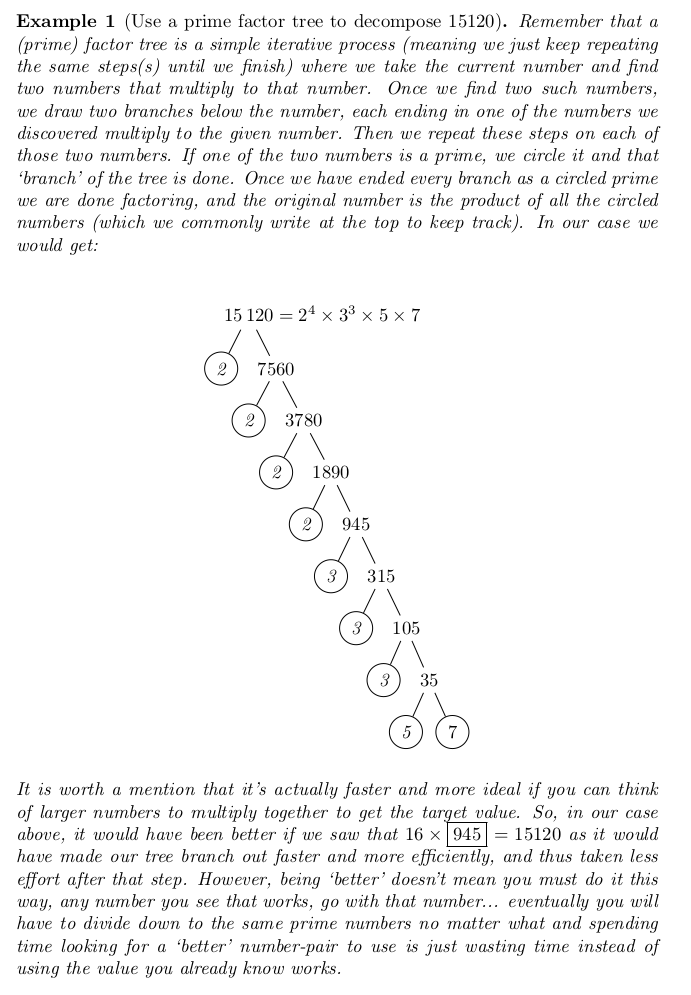
\includegraphics[width=\textwidth]{Ex1PrimeFactorTree.png}
%            \begin{forest}%
%                tikz={execute at end scope={\pgfmathparse{width("${}=\pt@result$")}%
%                    \path ([xshift=\pgfmathresult pt]pt-start.east);}},
%                [15120, start primeTree]
%            \end{forest}%%
%              \PrimeTree{15120}
        \end{center}
%\makeatother

%        It is worth a mention that it's actually faster and more ideal if you can think of larger numbers to multiply together to get the target value. So, in our case above, it would have been better if we saw that $16 \times \answer{945} = 15120$ as it would have made our tree branch out faster and more efficiently, and thus taken less effort after that step. However, being `better' doesn't mean you \textit{must} do it this way, any number you see that works, go with that number... eventually you will have to divide down to the same prime numbers no matter what and spending time looking for a `better' number-pair to use is just wasting time instead of using the value you already know works.
%    \end{example}% End prime factor tree box

    Now that we have the prime factorization we can continue to our example.

    \begin{example}
        
        {\bfseries Simplify the numeric root: $\sqrt[3]{15120}$}\\%
        Since we have already determined the prime factorization, we will write out our radical with the radicand in the factored form:
        \[
            \sqrt[3]{15120} = \sqrt[3]{2^4\times 3^3\times 5\times 7}
        \]
        As before, we want to group these terms as each factor to the root level ($3$ in this case) with remainders. Specifically we have $2^4 = (2^3)^1 \times 2^1$ and $3^3 = (3^3)^1 \times 3^0 = (3^3)^1$, and the $5$ and $7$ are both left alone (since they have powers less than $3$ to start with). So we would write;
        \[
            \sqrt[3]{2^4\times 3^3\times 5\times 7} = \sqrt[3]{(2^3)^1 \times 2^1 \times (3^3)^1\times 5\times 7}
        \]
        Then, pulling out the pieces that are grouped in the form $\text{(factor)}^{\text{(root value)}}$ (ie $\text{(factor)}^3$) we get:
        \[
            \sqrt[3]{(2^3)^1 \times 2^1 \times (3^3)^1\times 5\times 7} = \sqrt[3]{(2^3)^1\times (3^3)^1}\sqrt[3]{2^1 \times 5 \times 7}
        \]
        And, finally we can simplify the first cube root and combine the factors in the second cube root to get:
        \[
            \sqrt[3]{(2^3)^1\times (3^3)^1}\sqrt[3]{2^1 \times 5 \times 7} = (2 \times 3) \sqrt[3]{2\times 5 \times 7} 
                = \answer{6}\sqrt[3]{\answer{70}}
        \]

        And so we have our final simplified expression and we conclude:
        \[
            \sqrt[3]{15120} = \answer{6}\sqrt[3]{\answer{70}}
        \]
    \end{example}% End example.
%            
%
%
%\begin{question}
%    This is a purely Place Holder type question that will be replaced.
%    \begin{multipleChoice}
%        \choice{This question shouldn't be possible to get correct.}
%    \end{multipleChoice}
%\end{question}
%
%
%

\end{document}